\chapter{Modeling and Implementation}
\label{chapter:implementation}

\section{Overview}
As with the sequential implementation, the parallel implementation used the preprocessed terrain data to feed into the simulator. The kernels are written using the GPU programming language CUDA \cite{cuda}. CUDA is a parallel computing programming language designed to run on NVIDIA produced GPUs. CUDA allows GPUs to be used for general-purpose computing, and is therefore the ideal language with which to program a highly parallelized version of the fire propagation model. Three kernels were implemented for this paper, based on the three propagation methods presented in Section IV. An overall algorithm for the kernel calls is outlined in Algorithm \ref{alg:kernel}. The details on implementation of the kernels are found in the subsequent subsections.

\begin{algorithm}
  \small
  \caption{Simulation Composition}
  \label{alg:kernel}
  \begin{algorithmic}
  \WHILE{Simulation !Complete}
  \STATE computeKernel$<<<Blocks,Threads>>>$(inputs)
  \STATE terminateKernel$<<<Blocks,Threads>>>$(inputs)
  \ENDWHILE
  \end{algorithmic}
\end{algorithm}

The blocks and threads referenced in Algorithm \ref{alg:kernel} are referencing the blocks and threads that are allocated by the GPU upon initiation of the kernel. Each GPU has a specific number of blocks that it can allocate, and each block has a number of threads it can allocate. The threads process the kernel code independently of each other. Two kernels are necessary in this work because there is no way to force block-wise synchronization without a kernel finishing its work. The CPU calls the two kernels in a loop in this manner to ensure that one time step's propagation is calculated before the next can begin.

In order to address the runtime analysis needed for this paper, a sequential version of the kernels was also implemented. The equations and spread methodologies are the same between the kernels and the sequential implementation. However, many of the data concurrency problems were not a problem in the sequential version, and therefore some of the secondary kernels which will be addressed were not implemented in the sequential versions. The sequential implementations are not discussed in detail in this paper because they are not the main focus of the library and exist mostly for comparison purposes.  


\section{Surface Fire}
There are several potential approaches to calculating the propagation of the fire. This paper implemented three methods for iterating through a simulation to calculate the time of arrival map for a simple one-source forest fire under constant terrain and wind conditions. The first two spread methods (Minimal Time and Iterative Minimal Time) are based on stepping through time independent of specific fuel conditions and are based on the paper by Sousa, dos Reis, and Pereira \cite{gpufire}. The third spread method implemented in this paper (Burn Distances) was based on code and methods found in vFire \cite{vFire}. vFire implemented an accurate spread rate calculator based on Rothermel's fire spread equations and the fire spread and fuel model data to propagate based upon the physical burning of fuel.

The model for propagation rate used in this paper was the same for all three spread methods. The model is based on Rothermel's fire spread equations, and is found in Equation \ref{eq:rate}. This equation was derived by the creators of vFire \cite{vFire}, and the data processing done in the preprocessing phase of this project was based on their work. The preprocessing step translates the equation from Rothermel's work seen in Equation \ref{eq:roth} to what is seen in the following Equation \ref{eq:rate}. The preprocessing data is out of the scope of this paper and is not covered in detail. 

\begin{equation}
r(\Theta ) = R_{max}\frac{1.0 - \varepsilon }{1.0 - \varepsilon cos(\phi-\Theta )}
\label{eq:rate}
\end{equation}

$R_{max}$ is the maximum rate at which a fire can spread. $\varepsilon$ is the eccentricity of the fire, which is based on wind and slope data. $\phi$ is the orientation. $\Theta$ is the direction in which the fire is spreading. $R_{max}$, $\varepsilon$, and $\phi$ are all computed based on the terrain data before the propagation simulation takes place. This is done in the preprocessing stage because the rates at each cell do not change until the forest model changes. An interactive simulator could potentially allow for these variables to change (i.e. modeling a water dump from a helicopter or a bulldozer tearing down a line of trees) but that is outside the scope of this research paper. To implement these features, changes would be made to the fuel and moisture models used to determine the possible rate of change in a cell. The direction $\Theta$ is computed based on which neighbor is being examined at the time. 

During the preprocessing phase, there are several data files which need to be processed and interpolated to be of the same size. The fuel data and slope data are stored in files containing interpolation data such as size of cell, width, and height of the data grid. The Geospatial Data Abstraction Library (GDAL) was used to interpolate the data from the terrain and fuel files into the desired size of simulation \cite{GDAL}. Wind data is incorporated into the spread rate calculations as a 2D vector for each cell in the grid. The wind data contains a direction and magnitude. The fuel models provide the detailed parameters by which the rate of of spread is calculated. There are potential areas in this processing phase (such as calculating the Rothermel spread properties) that could be parallelized to improve overall running times of this simulator. However, the focus of this paper was to explore the potential for calculating fire spread on the GPU, so these possibilities were not addressed and are left for future work. 


\section{Fire Propagation}
\subsection{Overview}
In a wildfire spread simulation, there has to be a way to iterate through time and check for the propagation of the fire. This thesis implemented three such spread methods, which provide different fireline shapes as they move through the simulation. Each of the propagation methods are written as CUDA kernels \cite{cuda}. The implementation details of each unique method follow in this section of the paper. The following figure, Figure \label{fig:spreadTypes_2}, is a repeat of Figure \ref{fig:spreadTypes} for ease of reference to the reader. It depicts the neighbor access methods for the propagation methods.

\begin{figure}%[!t]
\centering
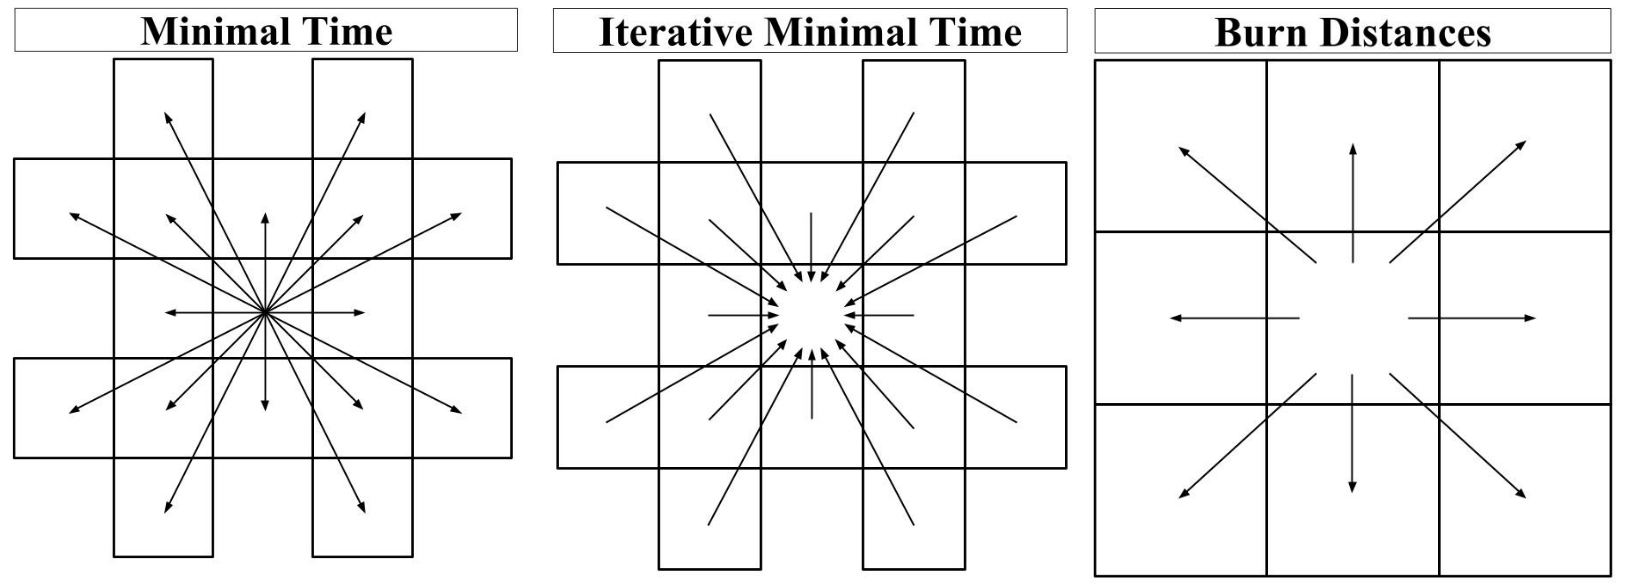
\includegraphics[width=\linewidth]{figures/background/spread_methods.PNG}
\caption{Neighbor access methodology for each of the propagation methods. From left to right: Minimal Time, Iterative Minimal Time, Burn Distances}
\label{fig:spreadTypes_2}
\end{figure}

\subsection{Burn Distances}
Burn distances is a kernel which simulates the burning of the physical distance between fire cells. In order to limit unnecessary computations, cells that are already on fire are skipped in the kernel. Only those that are not on fire check their neighbors to see if during this time step they are set alight.The pseudocode for the algorithm for the BD propagation method is found in Algorithm \ref{alg:BD}.

\begin{algorithm}[H]
  \caption{Burn Distances Algorithm}
  \label{alg:BD}
  \begin{algorithmic}
  \FOR{$cell = 0$ to $numCells$}
  \STATE $//$ Check to see not on fire
  \IF{$ignTime[cell] == INF$}
  \STATE $Skip$
  \ENDIF
  \STATE $//$ Check Neighbors for spread
  \FOR{$n = 0$ to $7$}
  \IF{$ignTime[neighborCell] < INF$}
  \STATE $Skip$
  \ENDIF
  \STATE $ROS$ = Compute ROS according to Equation \ref{eq:rate}
  \STATE $burnDistance$(totDist[neighborCell], ROS, timeStep)
  \IF{distance is burnt}
  \STATE $ignTime[neighborCell] = timeNow$
  \ENDIF
  \ENDFOR
  \ENDFOR
  \end{algorithmic}
\end{algorithm}

During each kernel call, each cell is processed independent of its neighbors. However, when a new cell ignites, the data must be written out to the vector somehow. There is no way to ensure which threads are reading and writing all at the same time. In fact, it was found that race conditions existed when the threads were reading from and writing to the same vector. In order to fix this problem, an input and output vector were created. Threads read only from the input vector and write to the output vector. A secondary kernel was written to copy the data values from one vector to another between the propagation kernel calls. The algorithm for the copy kernel may be found in Algorithm \ref{alg:BD_copy}:

\begin{algorithm}[H]
  \caption{Burn Distances Algorithm}
  \label{alg:BD_copy}
  \begin{algorithmic}
  \FOR{$cell = 0$ to $numCells$}
  \STATE $//$ Copy from output back to input 
  \STATE $InputVector[cell]$ = $OutputVector[cell]$
  \ENDFOR
  \end{algorithmic}
\end{algorithm}

An issue with this method arose from the static time step and needed to be addressed. Figure \ref{fig:accerr} shows the problem that can arise from the fixed time step. Figure \ref{fig:accerr} (a) shows the initial propagation. In this scenario, imagine that the propagation rate for b is much higher than a, but because the time step is large enough, they both propagate approximately one cell per time step. Figure \ref{fig:accerr} shows the second propagation step in time. In this example, a' propagates to a''. Because of the faster propagation rate of b, b' should propagate to b'' and b'' to b''' before a' propagates to a''. In the case where the time step is too large, the time of arrival would show an erroneous value for the cell holding a''. To fix this issue, the time step in the simulation must be set to a small enough value to avoid this error. The time step should be set to the smallest possible time it takes fire to propagate from one cell to another. 

\begin{figure*}
% \begin{figure}
\centering
%   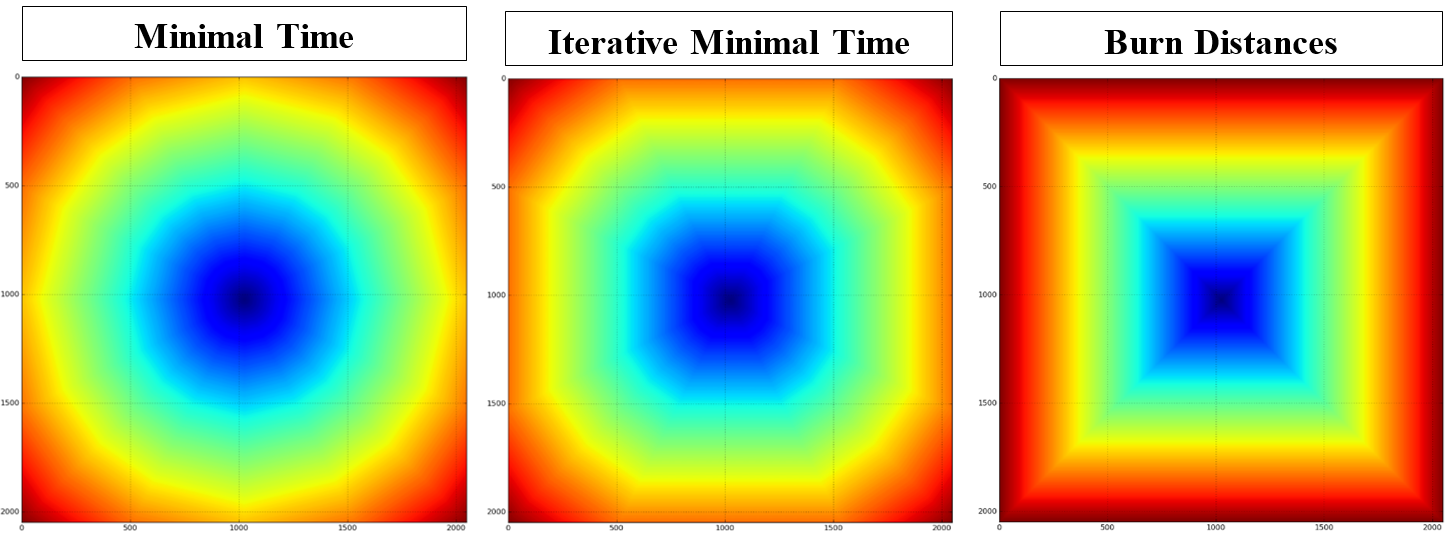
\includegraphics[width=\textwidth,height=4.2cm]{burn_patterns}
  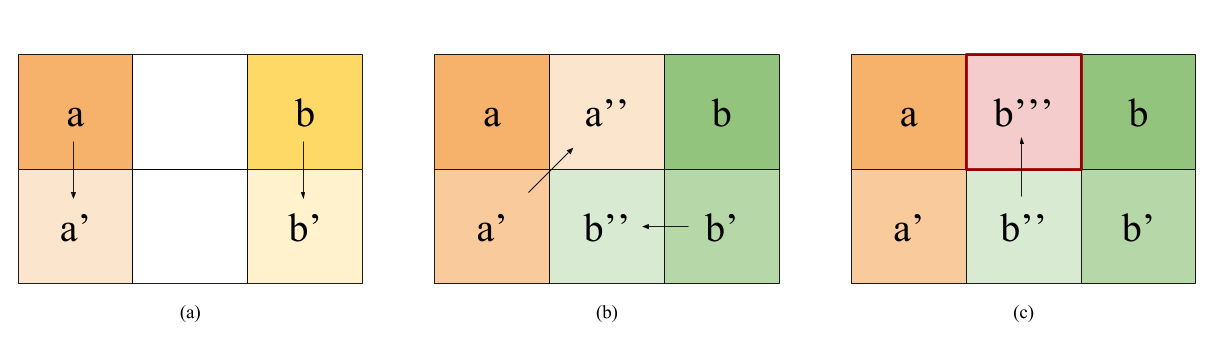
\includegraphics[width=\linewidth]{figures/implementation/Acceleration_error.png}
  \caption{The possible error for a fixed time-step propagation method. (a) shows the initial step with two lit cells a and b propagating to cells a' and b'. (b) shows a' propagating to a'' in the next time step. (c) is the situation where b'' would have propagated faster to the slot occupied in the previous step by a'', but because of the fixed time step, it would not propagate to an already lit cell.}
  \label{fig:accerr}
% \end{figure}
\end{figure*}eq:roth

A cell ignites when the distance from an ignited neighbor has been completely burned. Each cell stores the distance that has been consumed by the fire in each direction to its neighbors. The simulation checks a cell's neighbors for ignition, and then uses their properties to burn the amount of distance in that time step towards the current cell as seen in Figure \ref{fig:spreadTypes_2}. The cell ignites when one of its neighbors burns the distance completely. The cell then inherits the properties of the fire that propagated to it. The equation to determine how much distance is burned can be found in Equation \ref{eq:burn}. 

\begin{equation}
d = d - r \Delta t
\label{eq:burn}
\end{equation}

Where $d$ is the distance that needs to be consumed. It is slowly decremented over time by the rate of spread ($r$) times the time step size ($\Delta$ $t$). In order to account for the fact that an 'overburn' could occur with fixed time steps. The exact time of arrival that is calculated is dependent on the exact time of arrival that the fire would have arrived at the cell. The equation used to find the exact time of arrival is found in Equation \ref{eq:overburn}. eq:roth

\begin{equation}
TOA = t_{now} + \frac{d_{over}}{r}
\label{eq:overburn}
\end{equation}

Where $TOA$ is the time of arrival that is written out to the output time of arrival map, $t$ is the time in the simulation during which the propagation is occurring, $d_{over}$ is the distance the fire burnt past the desired difference, and $r$ is again the rate of spread. 

\subsection{Minimal Time}

The Minimal Time algorithm was developed using the information provided in Sousa, dos Reis, and Pereira's paper \cite{gpufire}. In this propagation method, each cell spreads outwards towards its neighbors. At each time step, a cell is examined to see if it is on fire. If the cell is burning, then it calculates the propagation time to the surrounding cells. If any of the neighbors are on fire, it is ignored. If the neighbor is unlit, then the time of arrival for that neighbor is calculated. A neighbor which has been lit in the same timestep as the current spread calculations will still be examined for the possibility of a sooner time of arrival from the current cell. A difference between this kernel and the Burn Distances kernel is the time stepping is dynamic. Each time a cell is successfully ignited, the new time of arrival is compared against a 'timeNext' variable to see if it a sooner time of arrival. The next step in time is based on the time in the simulation when the soonest cell ignites. The algorithm for the Minimal Time kernel may be found in Algorithm \ref{alg:MT}.

\begin{algorithm}[H]
%   \small
  \caption{Minimal Time Algorithm}
  \label{alg:MT}
%   \begin{algorithmic}[1] <- this will give you line number
  \begin{algorithmic}
  \FOR{$cell = 0$ to $numCells$}
  \IF{$timeNext > ignTime[cell] AND ignTime[cell] > timeNow$}
  \STATE $timeNext = ignTime[cell]$
  \ELSIF{$ignTime[cell] == timeNow$}
  \STATE $//$ Propagate Fire
  \FOR{$n = 0$ to $15$}
  \STATE $//$If neighbor is unburned
  \IF{$ignTime[neighborCell] > timeNow$}
  \STATE $ROS$ = Compute ROS according to Equation \ref{eq:rate}
  \STATE $ignTimeNew = timeNow + L_n / ROS$
  \IF{$ignTimeNew < ignTime[neighborCell]$}
  \STATE $igntime[neighborCell] = ignTimeNew$
  \ENDIF
  \IF{$ignTimeNew < timeNext$}
  \STATE $timeNext = ignTimeNew$
  \ENDIF
  \ENDIF
  \ENDFOR
  \ENDIF
  \ENDFOR
  \end{algorithmic}
\end{algorithm}

There are a few challenges which present themselves when implementing the algorithm. As in the Burn Distances kernel, data synchronization is an issue. Each cell in the fire is processed by one thread at a time, but every thread need access to the time of arrival map for both reading and writing. However, the solution to the problem between the two kernels is different. In order to minimize these race conditions, atomic operations were used to ensure that data integrity is maintained. CUDA's AtomicMin() operation was used to ensure that a cell that was writing to a data location was not overwriting a smaller time of arrival, which is the correct value that needed to be stored \cite{cuda}. Atomic operations in CUDA are designed to lock read-write access so a single thread has exclusive access rights. The AtomicMin() operation ensures that the minimum of two integers is the one which is stored at the memory location \cite{cudabyexample}. This solves the problem of one thread reading a value for its comparison then another writing a value to that same location, which would mean the value against which the calculations are compared would be inaccurate. A visual example of this read-write problem can be seen in Figure \ref{fig:readwrite}. The reason the AtomicMin() function is a solution to the read-write problem for this kernel as opposed to the Burn Distances kernel is that the Minimal Time Kernel processes integers. AtomicMin() has no implementation for floating point precision data values. 

\begin{figure}%[!b]
\centering
%   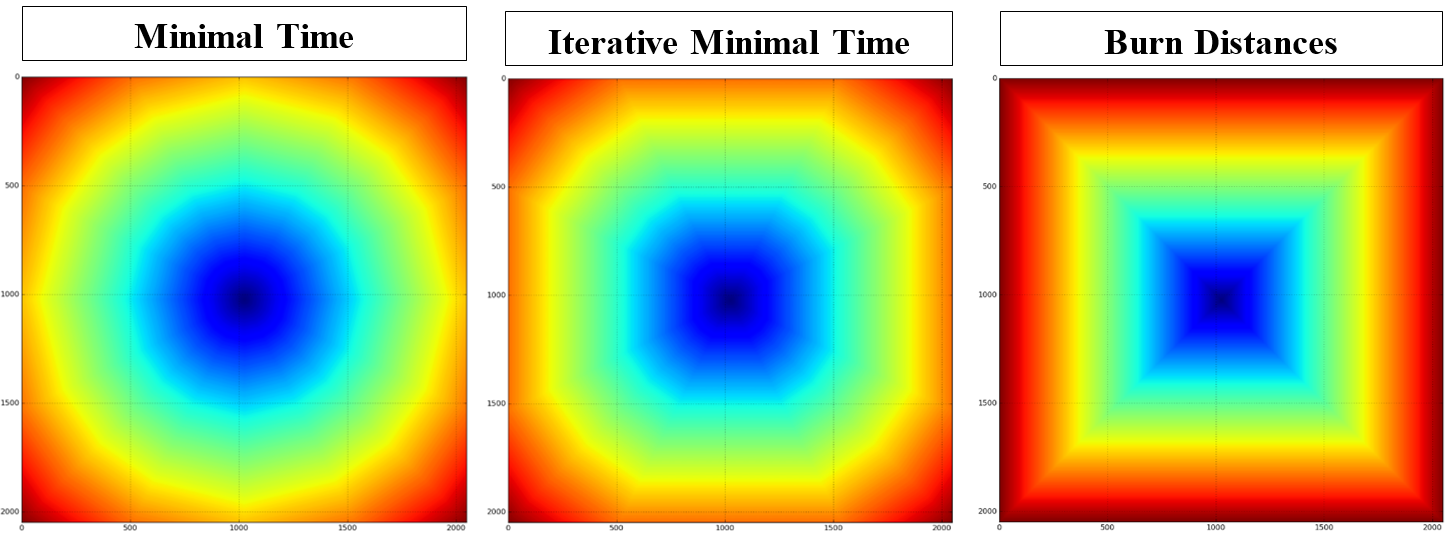
\includegraphics[width=\textwidth,height=4.2cm]{burn_patterns}
  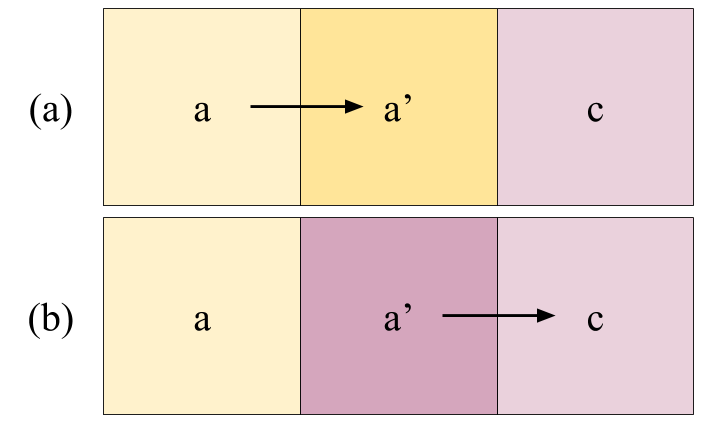
\includegraphics[height=4.2cm]{figures/implementation/read-write-issue.png}
  \caption{This is an example of the problem syncing thread read access and write access. There is no way to stop one thread writing to another cell before the value is read by another cell.}
  \label{fig:readwrite}
\end{figure}

A secondary kernel was introduced to manage the time update between time steps in the simulation. The secondary kernel was found to be the most efficient solution to this problem. CUDA does not allocate threads in any specific order, which means thread 1 could be the last to finish calculations while thread 1,000 could be the first \cite{cudabyexample}. In order to step through time in the MT propagation method, the timeNext variable needs to be updated after all calculations finish. Since there is no way to ensure which thread would be the last to finish operating on the data, another method for iterating the variable was needed after all threads had finished their computation. The secondary kernel is called after the first terminates, which ensures that all threads have finished their computation before the timeNext variable is updated. Copying the two-element time vector back to the host device and managing the update there was also tested, but it was found to be faster to write a new kernel to update the data without copying anything back to the host device.

\subsection{Iterative Minimal Time}
The parallel implementation of the IMT kernel is also very similar to the sequential implementation, and for the same reasons as the MT kernel pseudocode is not included, neither is IMT's. The same data synchronization issues are also found in this kernel, where reading from and writing to the same cells would cause race conditions. A simple example of this problem may be seen in Figure \ref{fig:readwrite}. There is no way to stop a thread from writing to an output position before another thread reads in the data it needs to do its own spread calculations. Figure \ref{fig:readwrite} (a) shows the writing of the value from a to a'. The value that existed before a' was the appropriate value for c to read in to do its calculations. Instead as seen in Figure \ref{fig:readwrite} (b), it is the result value from a that it reads into do its calculations. This error causes race conditions to occur and artifacts to appear in the simulation. Instead of using atomic operations to solve this problem, two time of arrival vectors are passed to the kernel at startup. The two kernels act as an input and output kernel, reading from the former and writing to the latter. This introduces a new problem with maintaining accurate spread data across the input and output vectors. The secondary kernel in the IMT method is both used to copy data from the output back into the input as well as checking for the terminating condition for the simulation. 

\begin{algorithm}[H]
%   \small
  \caption{Iterative Minimal Time Algorithm}
  \label{alg:IMT}
  \begin{algorithmic}
  \FOR{$cell = 0$ to $numCells$}
  \STATE $//$ Check for simulation completion:
  \IF{$|ignTime[cell] - ignTimeNext[cell]| < thresh$}
  \STATE $//$Mark as converged
  \ENDIF
  \IF{$ignTime[cell] > 0$}
  \STATE $ignTimeMin = INF$
  \STATE $//$Propagate Fire
  \FOR{$n = 0$ to $15$}
  \STATE $ROS$ = Compute ROS according to Equation \ref{eq:rate}
  \STATE $ignTimeNew = timeNow + L_n / ROS$
  \STATE $ignTimeMin = MIN(ignTimeNew, ignTimeMin)$
  \ENDFOR
  \ENDIF
  \ENDFOR
  \end{algorithmic}
\end{algorithm}

\section{Fire Acceleration}

\section{Crown Fire}

\section{Spotting}

\section{Simulation Progression}